\documentclass{article} % This command is used to set the type of document you are working on such as an article, book, or presenation

\usepackage{geometry} % This package allows the editing of the page layout
\usepackage{amsmath}  % This package allows the use of a large range of mathematical formula, commands, and symbols
\usepackage{graphicx}  % This package allows the importing of images

\newcommand{\question}[2][]{\begin{flushleft}\textbf{Question #1}: \textit{#2}\end{flushleft}}
\newcommand{\sol}{\textbf{Solution}:} %Use if you want a boldface solution line
\newcommand{\maketitletwo}[2][]{\begin{center}
        \Large{\textbf{Homework 1 Report}
        
            Reinforcement Learning} % Name of course here
        \vspace{5pt}
        
        \normalsize{
            Name: Kai-Jie Lin 
            
            Student ID: 110652019
            
            \today}
        \vspace{15pt}
        \end{center}}
\begin{document}
    \maketitletwo[5]  % Optional argument is assignment number
    %Keep a blank space between maketitletwo and \question[1]
    
    \section{Experiment}
    \subsection{Vanilla REINFORCE}
    Training result of the Vanilla REINFORCE. \\
    Hyperparameters: Learning rate = 0.001, decay rate of learning rate = 0.9, discounted factor = 0.999. \\
    Environment: Cartpole-v0.\\
    Result(EWMA reward): Converge in near 500 steps.\\
    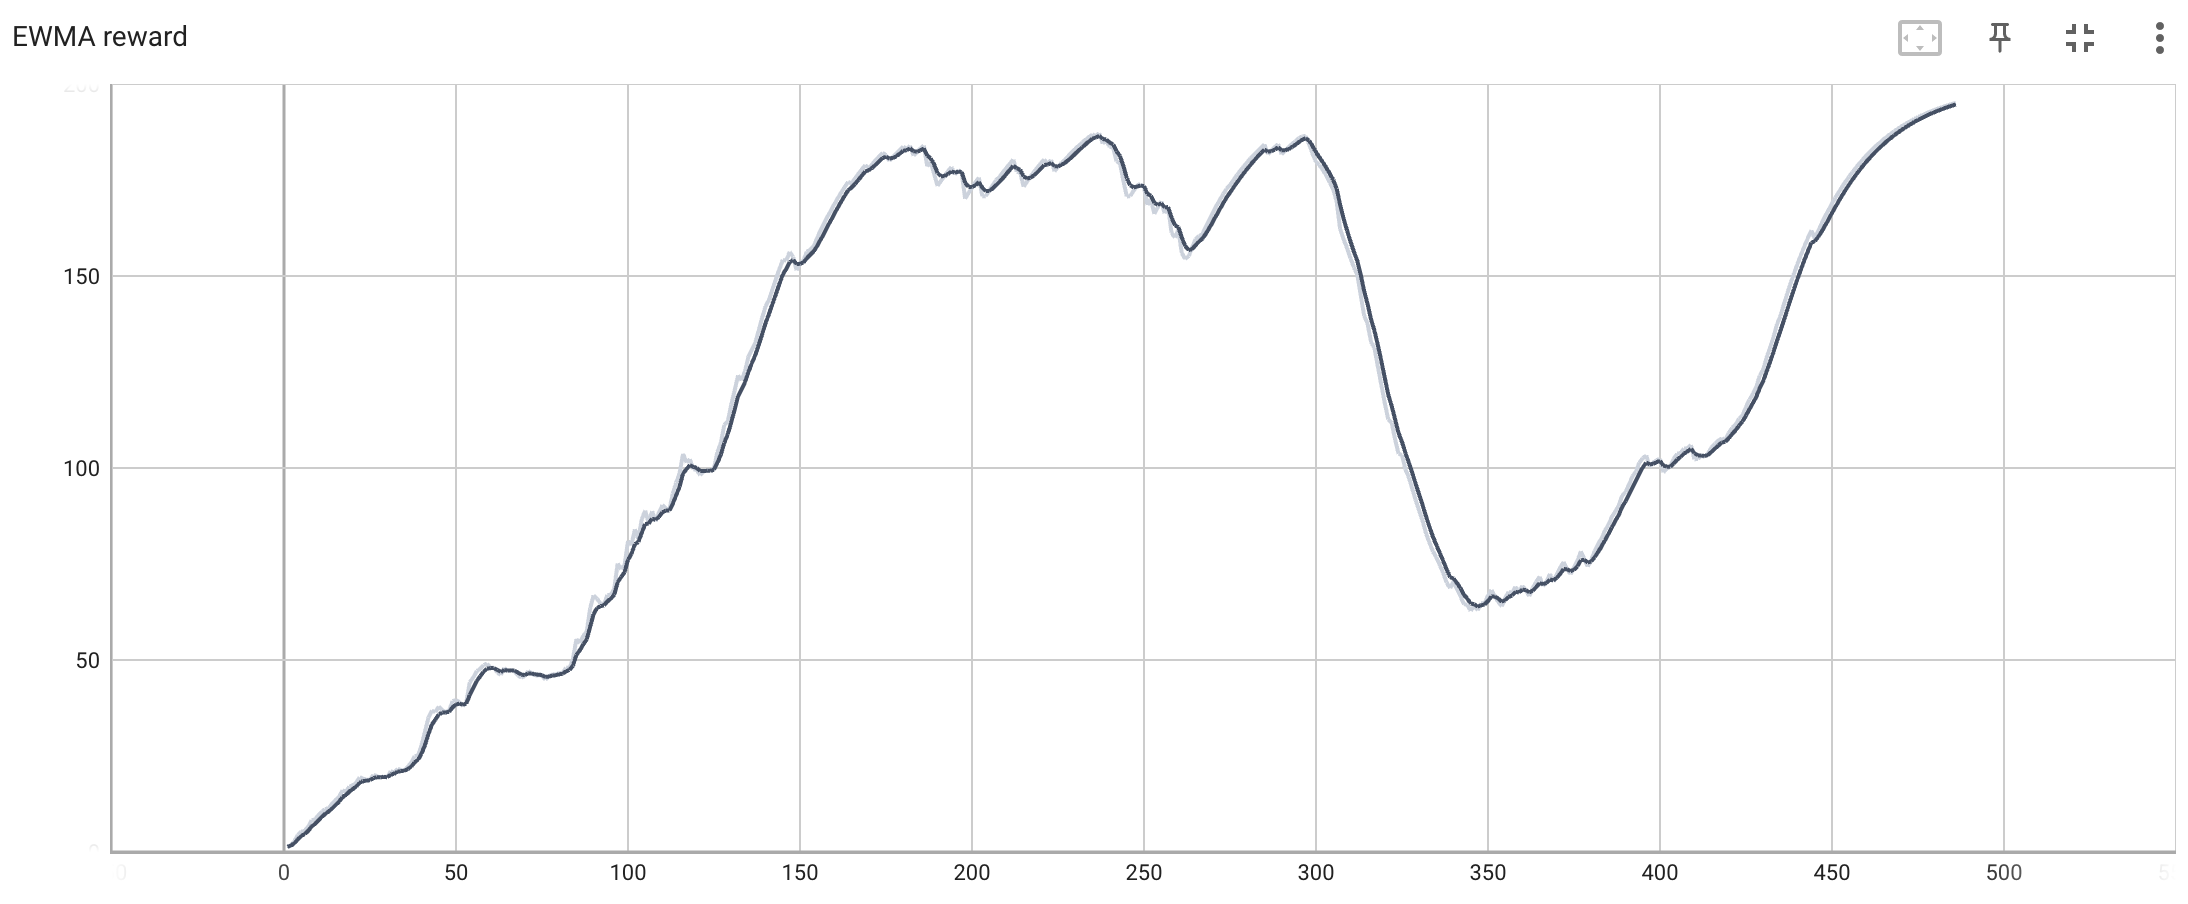
\includegraphics[width=10cm]{./imgs/vannila.png}
    \subsection{REINFORCE with baseline}
    Training result of REINFORCE with baseline. 
    Hyperparameters: Learning rate = 0.002, decay rate of learning rate = 0.95, discounted factor = 0.999. \\
    Environment: LunarLander-v2.\\
    Result(EWMA reward): Converge in 2037 steps.\\
    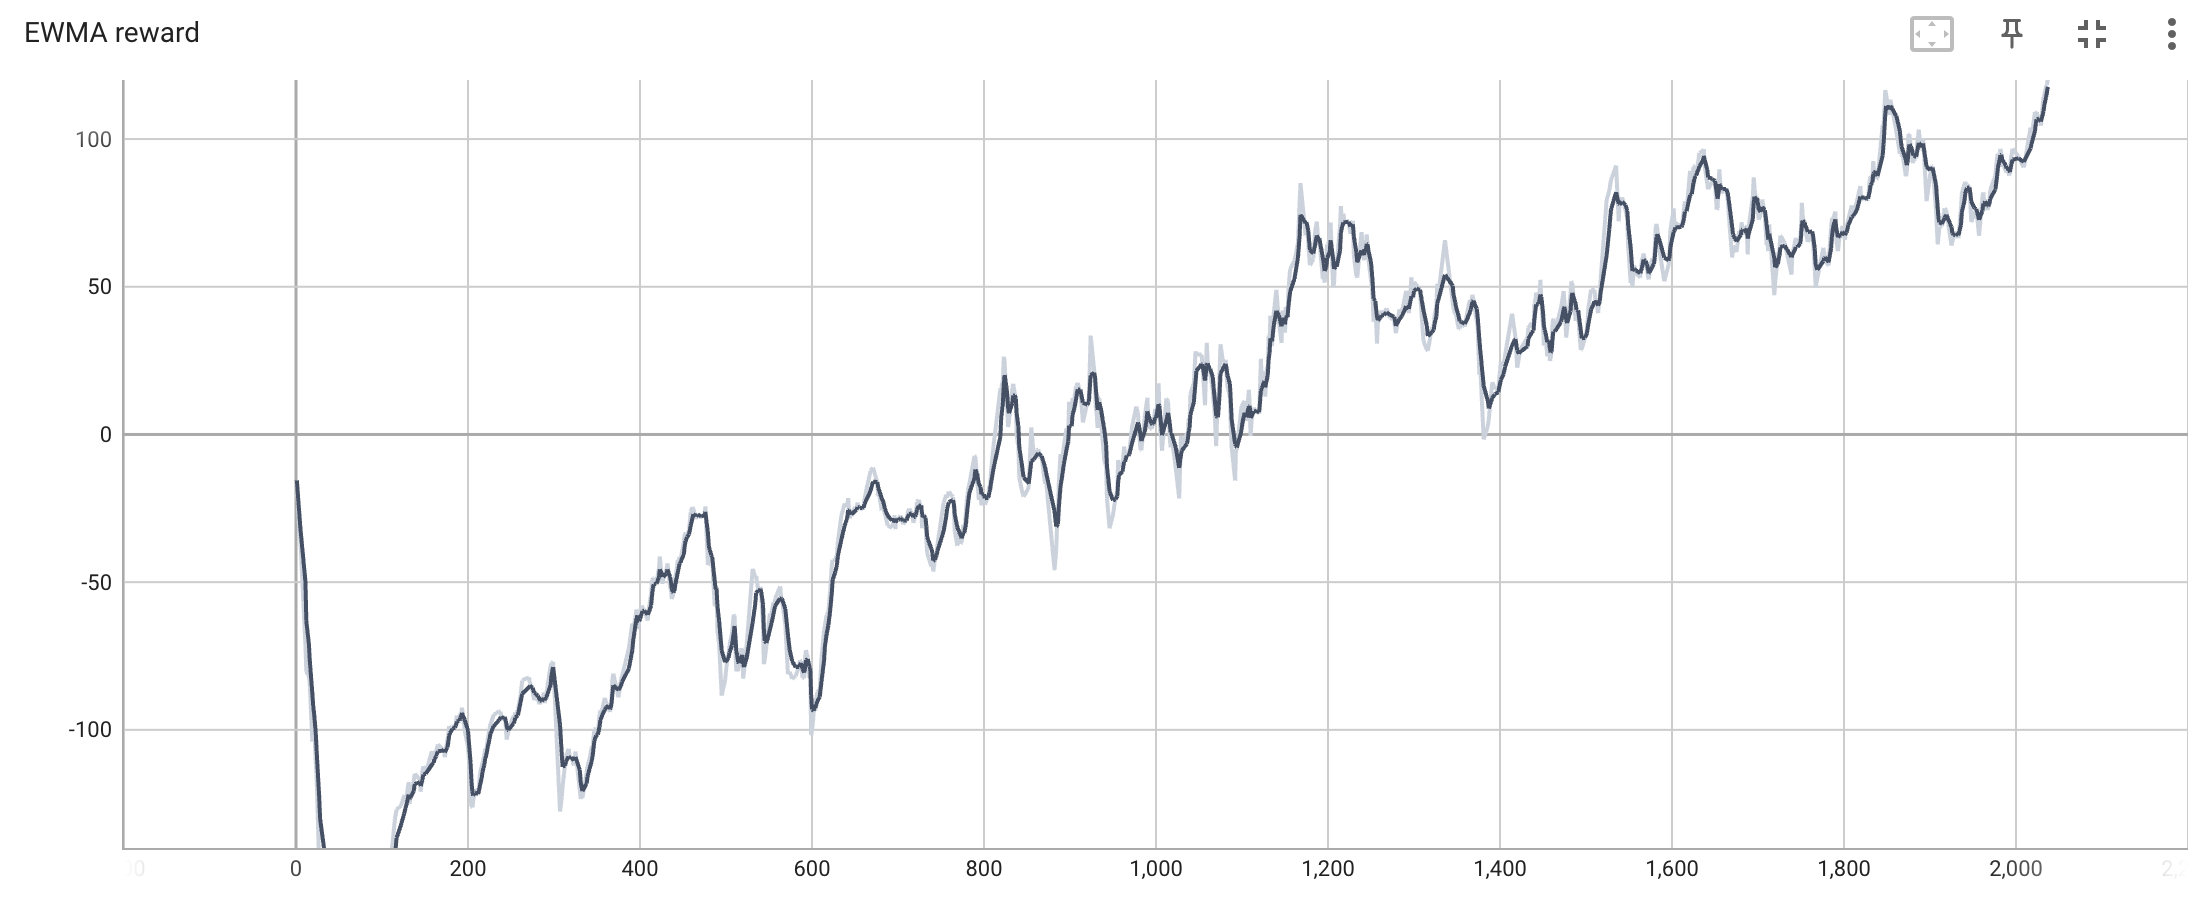
\includegraphics[width=10cm]{./imgs/baseline.png}
    \subsection{REINFORCE with GAE}
    Training result of REINFORCE with GAE. I have used bayesian optimization to tuning the hyper-parameters to reach better result.
    Bayesian optimization have tried 15 parameters combinations(learning rate, learning rate decay, lambda for GAE). The episodes would stop in 5000 steps once it have not converge to 120.
    Otherwise the running time will be too long. I have spent on this tuning process for 17 hours. All trajectory:\\
    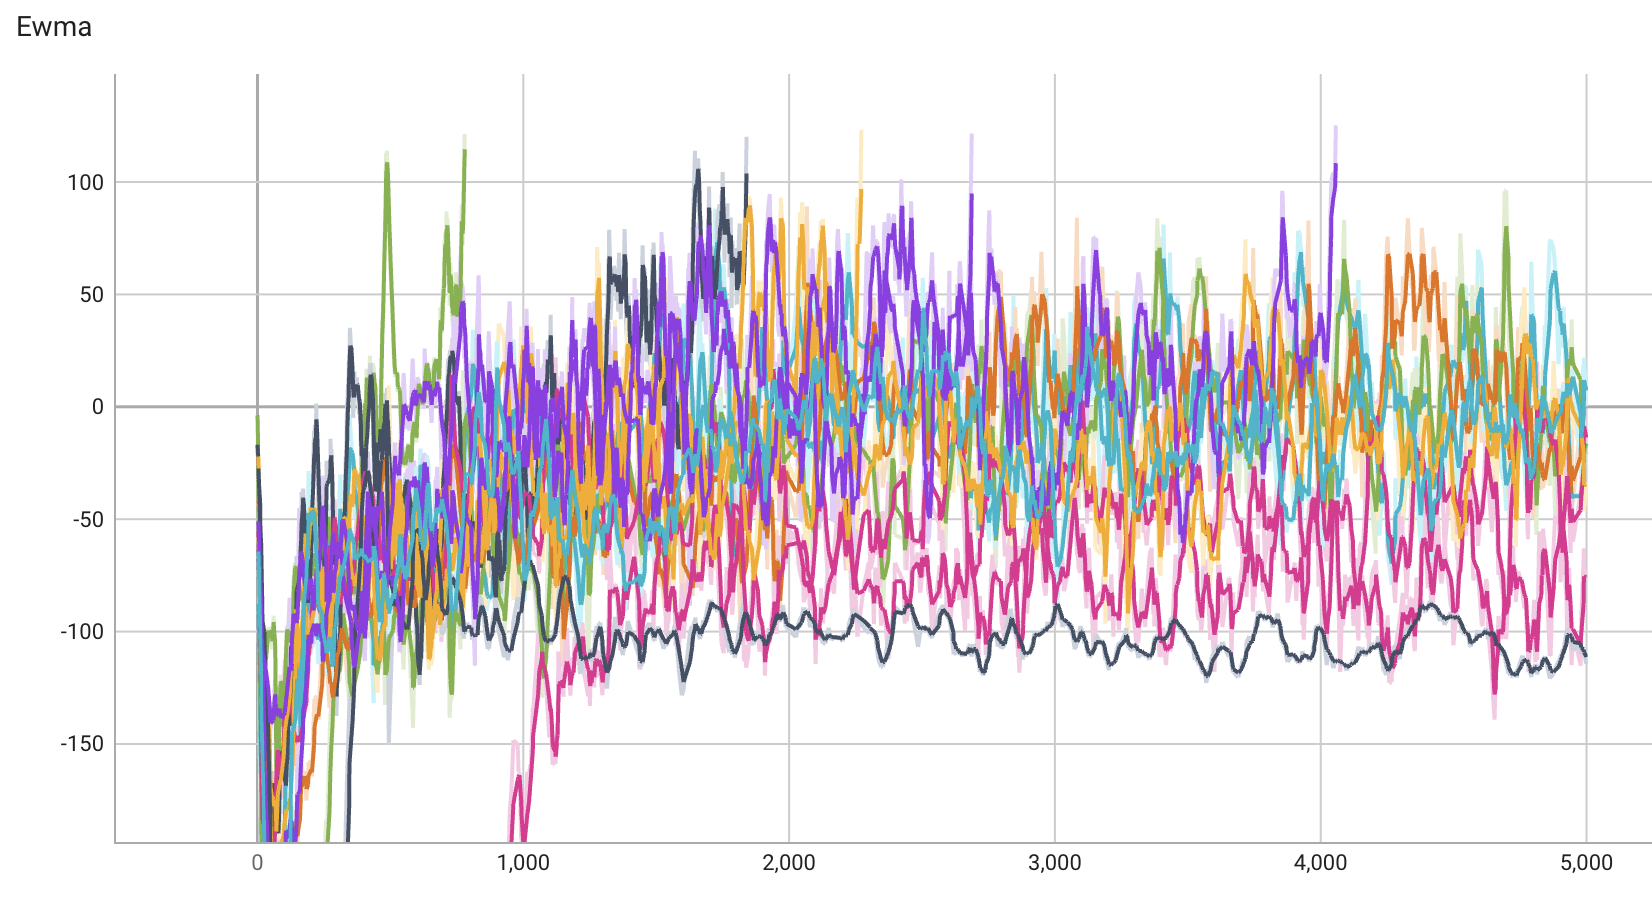
\includegraphics[width=10cm]{./imgs/all.png} \\
    I selected some of them which have converged to 120 EWMA reward and list below also for comparing the difference of different $\lambda$ (picture at the bottom): \\
    \begin{table}[h]
        \centering
        \begin{tabular}{|c|c|c|c|}
        \hline
        \textbf{Learning Rate} & \textbf{LR Decay} & \textbf{$\lambda$} & \textbf{Episodes spent} \\ \hline
        0.0065 & 0.8104 & 0.9700 & 780  \\ \hline
        0.0080 & 0.8561 & 0.7752 & 1840 \\ \hline
        0.0047 & 0.9436 & 0.6358 & 2272 \\ \hline
        0.0039 & 0.9508 & 0.5361 & 4057 \\ \hline
        \end{tabular}
        \caption{Hyperparameters and Results for REINFORCE with GAE}
        \label{tab:gae_results}
    \end{table}
    \\
    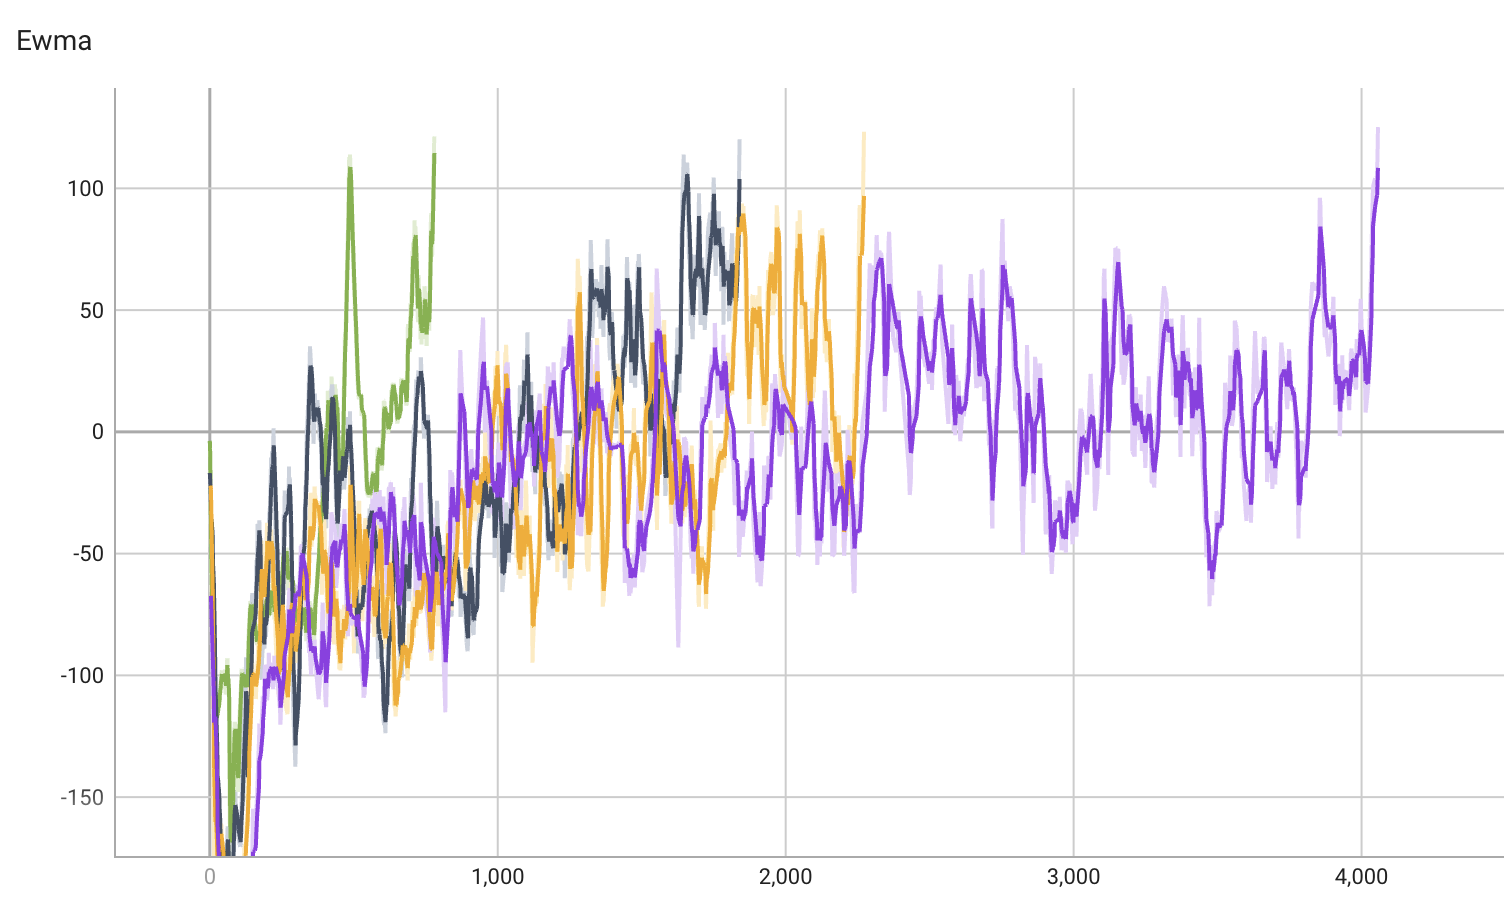
\includegraphics[width=10cm]{./imgs/four_line.png} \\
    
    \section{Discussion}
    \subsection{Neural Network}
    Three model used same architecture. 
    Two shared linear layer, one action layer and one value layer. 
    The activation function is ReLU. 
    The vannila version have hidden size 128. 
    Baseline and GAE version have hidden size 256.
    \subsection{Implementation of GAE}
    My implementation of GAE is nothing special. It is like the formula below:
    $$
    \hat{A}_t^{GAE(\gamma,\lambda)} = \sum_{k=0}^{\infty}{(\gamma \lambda)^k(\delta_{t+k})}
    $$
    $\hat{A}_t^{GAE(\gamma,\lambda)}$ is the GAE estimate of the advantage at time step $t$.
    $\gamma$ is the discount factor.
    $\lambda$ is the GAE parameter.
    $\delta_{t+k}$ is the temporal difference error at time step $t+k$, defined as $\delta_{t+k} = R_{t+k} + \gamma V(S_{t+k+1}) - V(S_{t+k})$, where $R_{t+k}$ is the reward received at time step $t+k$, $S_{t+k}$ is the state observed at time step $t+k$, and $V(s)$ is the value function estimated for state $s$.
    \subsection{About $\lambda$ in GAE}
    From the section 1.3, we can see that when $\lambda$ is large, the converge time is short, $\lambda$ is smaller, the converge time is longer.
    In my oppinion, since the reward distribution of environment LunarLander is farsighted, that is we need to sample whole trajectory to get important reward, thus the model sould consider more about the end of the trajectory.
    $\lambda$ controls how far we see the whole trajectory. When the $\lambda$ is large, the model may not be myopic.

\end{document}